\documentclass{beamer}
\usepackage{subcaption}
\usepackage{float}
\usepackage{setspace}
\usepackage{wrapfig}
\usepackage{caption}
\usepackage{mwe,tikz}\usepackage[percent]{overpic}
\captionsetup[figure]{labelformat=empty}
\usepackage{multirow}
\usepackage{array}
\usepackage{longtable}
\usepackage{pdfpcnotes}
\newcolumntype{L}[1]{>{\raggedright\let\newline\\\arraybackslash\hspace{0pt}}m{#1}}
\newcolumntype{C}[1]{>{\centering\let\newline\\\arraybackslash\hspace{0pt}}m{#1}}
\newcolumntype{R}[1]{>{\raggedleft\let\newline\\\arraybackslash\hspace{0pt}}m{#1}}
\usetheme[pageofpages=of,% String used between the current page and the
                         % total page count.
          bullet=circle,% Use circles instead of squares for bullets.
          titleline=true,% Show a line below the frame title.
          alternativetitlepage=true,% Use the fancy title page.
          titlepagelogo=logo-polito,% Logo for the first page.
          watermark=watermark-polito,% Watermark used in every page.
          watermarkheight=100px,% Height of the watermark.
          watermarkheightmult=4,% The watermark image is 4 times bigger
                                % than watermarkheight.
          ]{Theme}
\usepackage{lmodern}
\author{\small By\\Bharat Bhushan (153100048)}
\title{{{Thermoelastic fracture problems using Extended Finite\vspace{.3cm} Element Method}}}
\institute{\small Under the guidance of\\Prof. Salil S. Kulkarni\\ \vspace{5pt}Department of Mechanical Engineering, IIT Bombay}
\date{\vspace{-5pt}\today}
\begin{document}
%%%%%%%%%%%%%%%%%%%%%%%%%%%%%%%%%%%%%%%%%%%%%%%%%%%%%%%%%%%%%%%%%%%%5
%%%% TITLE PAGE %%%%%%%%%%%%%%%%%%%%%%%%%%%%%%%%%%%%%%%%%%%%%%%%%%%%
%%%%%%%%%%%%%%%%%%%%%%%%%%%%%%%%%%%%%%%%%%%%%%%%%%%%%%%%%%%%%%%%%%%%%
\begin{frame}[t,plain]
\titlepage
\end{frame}
%%%%%%%%%%%%%%%%%%%%%%%%%%%%%%%%%%%%%%%%%%%%%%%%%%%%%%%%%%%%%%%%%%%%%%
%%%% content %%%%%%%%%%%%%%%%%%%%%%%%%%%%%%%%%%%%%%%%%%%%%%%%%%%%%%%
%%%%%%%%%%%%%%%%%%%%%%%%%%%%%%%%%%%%%%%%%%%%%%%%%%%%%%%%%%%%%%%%%%%%

%%%%%%%%%%%%%%%%%%%%%%%%%%%%%%%%%%%%%%%%%%%%%%%%%%%%%%%%%%%%%%%%%
\begin{frame}[t,fragile]{Outline}
    \begin{itemize}
        \item Introduction 
        \item Motivation
        \item Literature Survey 
        \item Objectives  
        \item Computer implementation 
        \item Example problems
        \item Conclusion and future work
    \end{itemize}
\end{frame}
%%%%%%%%%%%%%%%%%%%%%%%%%%%%%%%%%%%%%%%%%%%%%%%%%%%%%%%%%%%%%%%%%
\begin{frame}[t,fragile]{Introduction: Thermo-elastic Fracture Mechanics}
    \vspace{-.3cm}
    \begin{itemize}
          \item Thermo-elastic Fracture mechanics is a field in which we Study the propagation of the crack in presence of temperature field.
                 \item Some application areas are as follows:
\begin{figure}[H]
      \begin{subfigure}{0.45\textwidth}
    \centering
     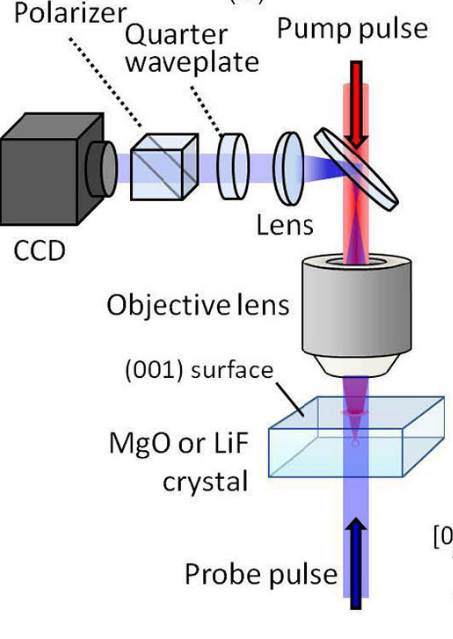
\includegraphics[scale=.1]{m}
 \vspace{-.2cm}
 \caption{\tiny Ultrafast laser}
 \end{subfigure}
\begin{subfigure}{0.45\textwidth}
    \centering
     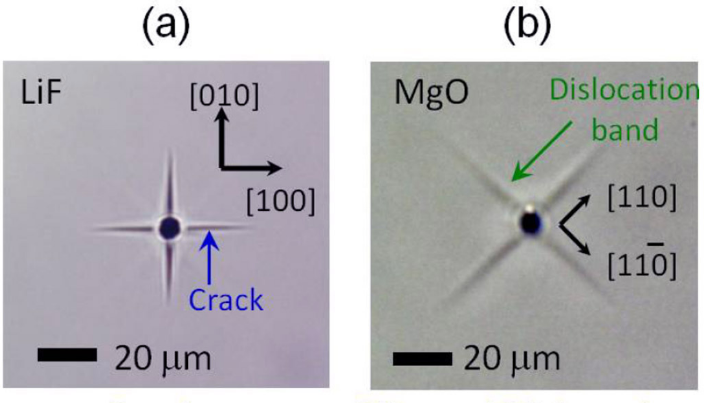
\includegraphics[scale=.1]{l}
 \vspace{-.2cm}
 \caption{\tiny Cracks generated in material}
 \end{subfigure}
       \vspace{-.3cm}
      \begin{subfigure}{0.45\textwidth}
    \centering
     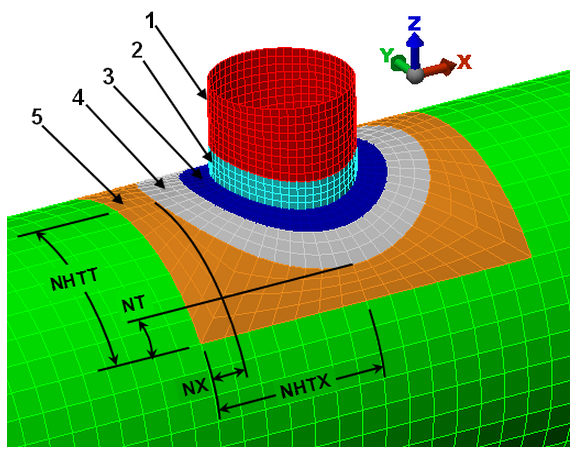
\includegraphics[scale=.1]{cyl.png}
 \vspace{-.2cm}
 \caption{\tiny{The cylinder-nozzle intersection.}}
 \label{cyl}
 \end{subfigure}
\begin{subfigure}{0.45\textwidth}
    \centering
     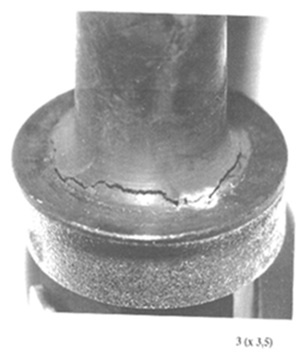
\includegraphics[scale=.1]{fail.jpg}
 \vspace{-.2cm}
 \caption{\tiny{Cracked baffle bolt of Belgian Nuclear Reactor}}
 \end{subfigure}
 \end{figure}
 \end{itemize}
 \vspace{.1cm}
   \tiny
   \hspace{15pt}
     \textbf{source}: Tian, X., Shen. (2006). A direct finite element method study of generalized thermoelastic problems. \\
   \vspace{-7pt}
   \hspace{15pt}
   \emph{International Journal of Solids and Structures}, 43(7), 2050-2063.
\end{frame}
%%%%%%%%%%%%%%%%%%%%%%%%%%%%%%%%%%%%%%%%%%%%%%%%%%%%%%%%%%%%%%%%%o 
\begin{frame}[t,fragile]{Motivation}
    \vspace{-.3cm}
    \footnotesize
\begin{itemize}
     \item Atkinson has solved a Dirichlet problem for Laplace's equation on a pie shaped region as:\vspace{-.2cm}
         $$u(x,y)= r^{\frac{\pi}{\phi}}\sin\alpha\theta,\  r>0,\ 0<\theta<\phi$$
        \vspace{-.6cm}
        \begin{itemize}
                \footnotesize
     \item Case I: $0<\phi<\pi$:
        $u'$ is continuous as we approach towards the origin 
     \item Case II: $\pi<\phi<2\pi$:
        $u'$ is not continuous as (x,y) approaches the origin 
    \end{itemize}
     \item When $\phi=2\pi$, the problem becomes a crack problem:
    \vspace{-.1cm}$$u \propto r^{\frac{1}{2}}\text{ and} \ u'\propto  r^{-\frac{1}{2}}$$ 
    \vspace{-.4cm}
     \item Substituting T in place of u: 
       $T \propto r^{\frac{1}{2}}\text{ and} \ T'\propto  r^{-\frac{1}{2}}$ 
    \item Thus, around the crack tip, thermal stresses also has square root singularity : our motivation for analyzing a thermo-elastic crack problem. 
\end{itemize}
  \tiny
  \vspace{10pt}
  \hspace{10pt}
    \textbf{source}: Atkinson, K. E. (1997).
    \emph{The numerical solution of \\
  \hspace{10pt}
    integral equations of the second kind} (Vol. 4). \\
  \hspace{10pt}
    Cambridge university press.
\begin{wrapfigure}{r}{0.4\textwidth}
    \centering
    \vspace{-55pt}
     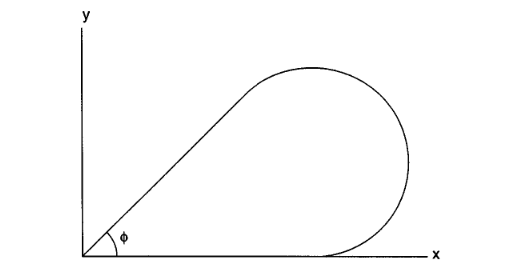
\includegraphics[width=.3\textwidth]{pie.png}
    \vspace{-8pt}
    \caption{\footnotesize Pie-shaped region.}
\end{wrapfigure}
\end{frame}
%%%%%%%%%%%%%%%%%%%%%%%%%%%%%%%%%%%%%%%%%%%%%%%%%%%%%%%%%%%%%%%%%%%%
\begin{frame}[t,fragile]{Introduction to Extended Finite Element Method }
    \begin{figure}
    \vspace{-.5cm}
        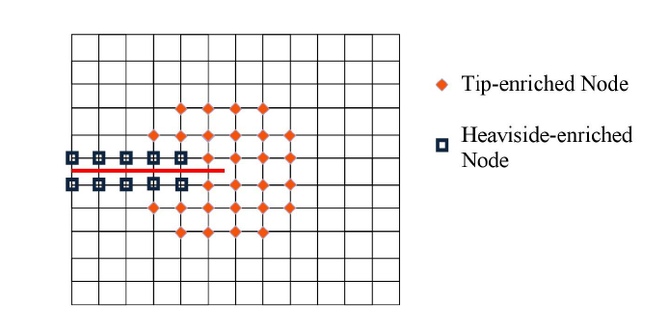
\includegraphics[scale=.2]{enrich.png}
    \vspace{-.4cm}
     \caption{\hspace{-1.5cm}\tiny X-FEM enrichment strategy}
\end{figure}
    \vspace{-.5cm}
\footnotesize
       $Heavyside \ enrichment\  functions:\ \ \ \ \ h(x,y)=\begin{cases}1,&       for ~ ~ y\ge 0\\ -1,&       for~ ~ y\le 0\end{cases}$\\ 
    \vspace{.2cm}
         $ u^h=\sum_i N_i(x)u_i+\sum_{j\in J} N_j(x) h(x)a_j+\sum_{k\in K} N_k(x)\left( \sum_{l=1}^{4}\gamma_l(x)b_{kl} \right)$\\
    \vspace{.2cm}
        $ v^h=\sum_i N_i(x)v_i+\sum_{j\in J} N_j(x) h(x)c_j+\sum_{k\in K} N_k(x)\left( \sum_{l=1}^{4}\gamma_l(x)d_{kl} \right) $\\
    \vspace{.2cm}
        where,$\gamma=\left[ \sqrt{r}\cos \left( \frac{\theta}{2} \right), \sqrt{r}\sin\left( \frac{\theta}{2} \right),\sqrt{r}\sin\left( \frac{\theta}{2} \right)\sin(\theta),\sqrt{r}\cos\left( \frac{\theta}{2} \right)\sin(\theta)\right] $\\
\tiny
    \vspace{.3cm}
\hspace{10pt}
     \textbf{Source:}Belytschko, T., \& Black, T. (1999). Elastic crack growth in finite elements with minimal remeshing. \\
\vspace{-7pt}
\hspace{10pt}
\emph{International journal for numerical methods in engineering}, 45(5), 601-620.
\end{frame}
%%%%%%%%%%%%%%%%%%%%%%%%%%%%%%%%%%%%%%%%%%%%%%%%%%%%%%%%%%%%%%%%%%%%%%%%
\begin{frame}[t,fragile]{Objectives: }
    \begin{itemize}
            \item Finite element formulation of semi-coupled thermoelasticity and implementation in MATLAB
            \item Validation of FEM programs by performing patch tests.
                      \item Development of Extended Finite Element Program for coupled thermoelastic fracture problems 
                      \item Utilization of the developed X-FEM Program in other fields which is governed by Laplace's equation
                \end{itemize}
\end{frame}
%%%%%%%%%%%%%%%%%%%%%%%%%%%%%%%%%%%%%%%%%%%%%%%%%%%%%%%%%%%%%%%%%%%
\begin{frame}[t,fragile]{Finite Element Formulation of Thermoelasticity}
    \vspace{-.4cm}
    \begin{itemize}      
\item A semi-coupled thermoelasticity problem is formulated.      
\item In semi-coupled problems we neglected the effect of displacements on temperature field.      
\item In presence of temperature field, the Hooke's law can be given by: 
    \footnotesize
\begin{align*}
    \begin{Bmatrix}
        \sigma_{x}\\ \sigma_{y}\\ \tau_{xy} 
    \end{Bmatrix} =\frac{E}{(1-\nu^2)}
    \begin{bmatrix}
        1 & \nu & 0 \\ \nu & 1 & 0 \\ 0 & 0 & 1-\nu 
    \end{bmatrix}
    \begin{Bmatrix}
        \varepsilon_{x}-\alpha\Delta T \\ \varepsilon_{y}-\alpha \Delta T \\ \varepsilon_{xy} 
    \end{Bmatrix}
\end{align*}
     
    \item The governing equations of the thermoelasticity are derived as follows: 
            \bgroup
            \begin{align*}
    \frac{\partial}{\partial x}\left[c_{11}\frac{\partial u}{\partial x}+c_{12}\frac{\partial v}{\partial y}\right]+&\frac{\partial}{\partial y}\left[c_{66}\left(\frac{\partial u}{\partial y}+\frac{\partial v}{\partial x}\right)\right]-(c_{11}+c_{12})\alpha\frac{\partial T}{\partial x}-f_x   =0 \\
    \frac{\partial}{\partial x}\left[c_{66}\left(\frac{\partial u}{\partial y}+\frac{\partial v}{\partial x}\right)\right]+&\frac{\partial}{\partial y}\left[c_{12}\frac{\partial u}{\partial x}+c_{22}\frac{\partial v}{\partial y}\right]-(c_{11}+c_{12})\alpha\frac{\partial T}{\partial y}-f_y=0\\
    &\ \ \ \ \ \ \ k\left( \frac{\partial^2 T}{\partial x^2}+\frac{\partial^2 T}{\partial y^2} \right)=q
\end{align*}
\egroup
       \end{itemize}
\end{frame}
%%%%%%%%%%%%%%%%%%%%%%%%%%%%%%%%%%%%%%%%%%%%%%%%%%%%%%%%%%%%%%%%%%%%%%
\begin{frame}[t,fragile]{Weak Form Equations of Coupled Thermoelasticity}
    \vspace{-.4cm}
            \scriptsize
            \begin{align*}
    -\int_{\Omega}^{}\left[ c_{11}\frac{\partial N_i}{\partial x}\frac{\partial N_j}{\partial x}u_j+c_{12}\frac{\partial N_i}{\partial x}\frac{\partial N_j}{\partial y}v_j\right]dxdy+\int_{\Omega}^{}\left[c_{66}\frac{\partial N_i}{\partial y}\frac{\partial N_j}{\partial y}u_jdxdy+\frac{\partial N_i}{\partial y}\frac{\partial N_j}{\partial x}v_j\right]dxdy\nonumber\\ -\int_{\Omega}^{}\frac{\partial N_i}{\partial x}\beta N_jT_j dxdy +\int_{\Omega}^{}N_if_x
     dxdy+\int_{\Gamma}^{}N_i\vec{t}dx=0\end{align*}
    \begin{align*}
     -\int_{\Omega}^{}\left[ c_{11}\frac{\partial N_i}{\partial y}\frac{\partial N_j}{\partial y}v_j+c_{12}\frac{\partial N_i}{\partial y}\frac{\partial N_j}{\partial x}u_j\right]dxdy+\int_{\Omega}^{}\left[c_{66}\frac{\partial N_i}{\partial x}\frac{\partial N_j}{\partial x}v_jdxdy+\frac{\partial N_i}{\partial x}\frac{\partial N_j}{\partial y}u_j\right]dxdy\nonumber\\ -\int_{\Omega}^{}\frac{\partial N_i}{\partial y}\beta N_jT_j dxdy+\int_{\Omega}^{}N_if_y dxdy+\int_{\Gamma}^{}N_i\vec{t}dy=0
 \end{align*}
      \begin{align*}
      k\int_{\Omega}\left( \frac{\partial N_i}{\partial x}\frac{\partial N_j}{\partial x}+\frac{\partial N_i}{\partial y}\frac{\partial N_j}{\partial y} \right)T_jdxdy-\int_{\Omega}^{}N_iN_jqdxdy=\int_{\Gamma}^{}N_i\bar{Q}ds& \end{align*}
\end{frame}
%%%%%%%%%%%%%%%%%%%%%%%%%%%%%%%%%%%%%%%%%%%%%%%%%%%%%%%%%%%%%%%%%%%
\begin{frame}[t,fragile]{Finite Element Model}
    \vspace{-.3cm}
    \footnotesize
    \begin{itemize}
          \item Neglecting the body forces, above equations can be written in matrix form as: 
    \begin{align*}
\begin{bmatrix}
    K_{11} & K_{12} \\
    0 & K_{22}
\end{bmatrix}
\begin{Bmatrix}
    U^e\\ T^e
\end{Bmatrix}=
\begin{Bmatrix}
    F\\ Q
\end{Bmatrix}
\end{align*}  
Where,
\vspace{-.2cm}
    \scriptsize 
\begin{align*}
    [K_{11}^e]=\int_{\Omega}[B]^T[C][B]dxdy\ \
    [K_{12}^e]=\int_{\Omega}[B]^T[\beta][N^{\theta}]dxdy\ \
    [K_{22}^e]=\int_{\Omega}[B^{\theta}]^T[K][B^{\theta}]dxdy
\end{align*}
\vspace{-.5cm}
\begin{align*}
    \{F\}=\int_\Gamma [N]^T{\bar{t}}ds\ \
    \{Q\}=\int_\Gamma [N^{\theta}]^T\bar{Q}ds
\end{align*}  
\item \large{Computer implementation:}
    \begin{itemize}
\footnotesize
         \item A MATLAB program is developed to solve the 2-dimensional thermoelasticity problems based on above Finite Element model 
         \item 4-noded quadrilateral (Q4) elements and 3-degrees of freedom per node 
         \item  $2\times 2$ Gauss quadrature rule is used for numerical integration
    \end{itemize}
\end{itemize}
\end{frame}
%%%%%%%%%%%%%%%%%%%%%%%%%%%%%%%%%%%%%%%%%%%%%%%%%%%%%%%%%%%%%%%%%%%%%%%%%
\begin{frame}[t,fragile]{Patch Test 1: Validation of Elasticity code}
    \vspace{-.4cm}
    \footnotesize
 \begin{itemize}
        \item A square plate is taken and meshed with 5 elements as shown in the figure below. 
            \item Minimum number of essential boundary conditions is fixed to eliminate the rigid body motions
            \item Loads are applied such that there is constant state of stress in the body
            \item Numerical integration is performed using $2\times 2$ Gauss quadrature rule.
   \end{itemize}
   \vspace{-.5cm}
    \begin{figure}
\begin{subfigure}{0.45\textwidth}
    \centering
       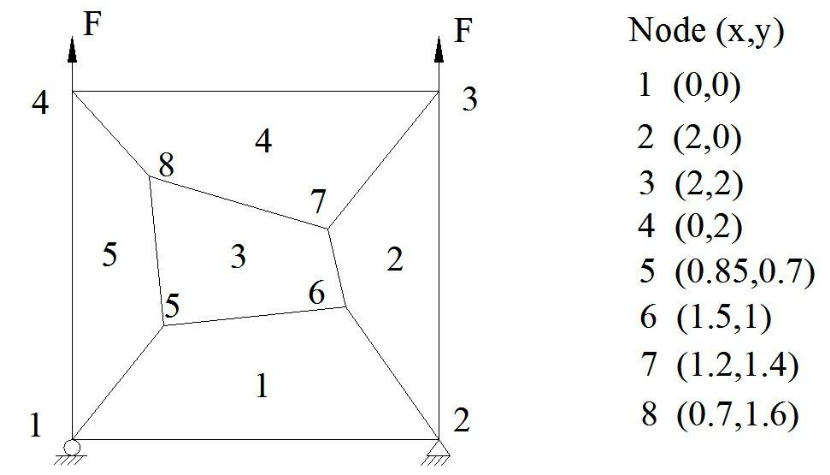
\includegraphics[scale=.2]{image2}
    \caption{\scriptsize Mesh Configuration }
\end{subfigure}
\begin{subfigure}{0.45\textwidth}
     \centering   
    \vspace{-2pt}
\caption{\scriptsize Results of Patch Test }
    \vspace{-4pt}
 \scalebox{.5}{\begin{tabular}{|c|c|c|c|c|}
\hline
& Gauss Point& $\sigma_x/F$ & $\sigma_y/F$ & $\tau_{xy}/F$\\
\hline
\multirow{4}{5em}{Element 1} & 1 & $0.166\times 10^{-15}$ &1& $0.1665\times 10^{-15}$\\
& 2 & $-0.033\times 10^{-15}$ &1& $0.1665\times 10^{-15}$\\
& 3 & $-0.063\times 10^{-15}$ &1& $0.222\times 10^{-15}$\\
& 4 & $0$ &1& $0$\\
\hline
\multirow{4}{5em}{Element 2} & 1 & $0.062\times 10^{-15}$ &1& $0$\\
& 2 & $-.41633\times 10^{-15}$ &1& $-0.222\times 10^{-15}$\\
& 3 & $0.02775\times 10^{-15}$ &1& $0.138\times 10^{-15}$\\
& 4 & $-0.2220\times 10^{-15}$ &1& $0$\\
\hline
\multirow{4}{5em}{Element 3} & 1 & $0.222\times 10^{-15}$ &1& $0.1665\times 10^{-15}$\\
& 2 & $0.0555\times 10^{-15}$ &1& $0.222\times 10^{-15}$\\
& 3 & $-0.0555\times 10^{-15}$ &1& $0$\\
& 4 & $0.22204\times 10^{-15}$ &1& $0$\\
\hline
\multirow{4}{5em}{Element 4} & 1 & $-0.222\times 10^{-15}$ &1& $0.1665\times 10^{-15}$\\
& 2 & $0.222\times 10^{-15}$ &1& $0.1665\times 10^{-15}$\\
& 3 & $-0.063\times 10^{-15}$ &1& $0.222\times 10^{-15}$\\
& 4 & $0.222\times 10^{-15}$ &1& $0$\\
\hline
\multirow{4}{5em}{Element 5} & 1 & $-0.422\times 10^{-15}$ &1& $0.1665\times 10^{-15}$\\
& 2 & $0.222\times 10^{-15}$ &1& $0.1665\times 10^{-15}$\\
& 3 & $-0.063\times 10^{-15}$ &1& $0.222\times 10^{-15}$\\
& 4 & $0.222\times 10^{-15}$ &1& $0$\\
\hline
\end{tabular}}
     \end{subfigure}
  \end{figure}
\end{frame}
%%%%%%%%%%%%%%%%%%%%%%%%%%%%%%%%%%%%%%%%%%%%%%%%%%%%%%%%%%%%%%%%%%%%%%%%%%%%
\begin{frame}[t,fragile]{Patch Test 2: Validation of Thermoelasticity code}
    \vspace{-.5cm}
    \scriptsize  
\begin{figure}[H]
    \centering
     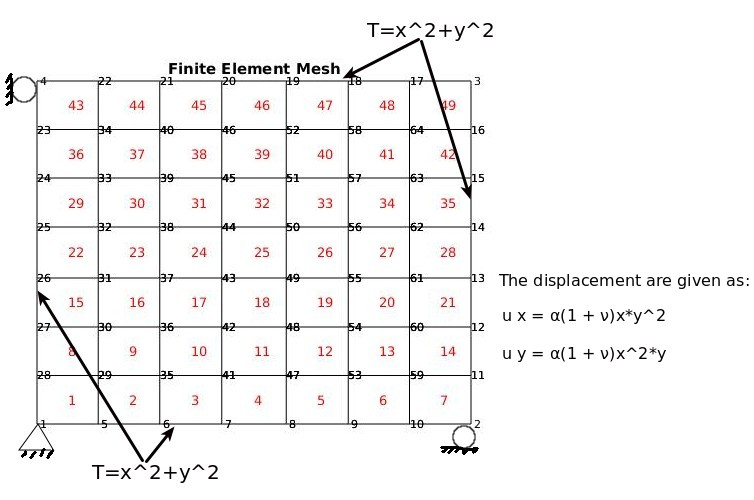
\includegraphics[scale=.20]{elements_7^2_1.jpg}
\end{figure}
   \vspace{-.5cm}
\begin{itemize}
       \item A temperature distribution of $T=x^2+y^2$ is applied on 4 boundaries of plate which satisfies the Poisson's equation $\frac{\partial^2 T}{\partial x^2}+\frac{\partial^2 T}{\partial y^2}=4$. 
       \item Heat source $q=4$ is applied throughout the body. 
       \item Results are compared with the analytical solutions in the following table:
\end{itemize}
\vspace{-10pt}
\bgroup
\begin{table}[H]
    \centering
    \begin{tabular}{|C{1cm}|C{4cm}|C{4cm}|}
\hline 
Nodes& \% \ Error in Temperature T&\% Error in displacement $u_y$\\
\hline
30 & -0.0523342237$\times 10^{-12}$&0.00034894013\\
\hline
33 & 0.1046684475$\times 10^{-12}$&0.00082764871\\
\hline
63 & 0.0916486147$\times 10^{-12}$&0.00015321553\\
\hline
\end{tabular}
\end{table}
\egroup

 
\end{frame}
%%%%%%%%%%%%%%%%%%%%%%%%%%%%%%%%%%%%%%%%%%%%%%%%%%%%%%%%%%%%%%%%%%%%%%%%%%
\begin{frame}[t,fragile]{Mesh Refinements}
     
      \vspace{-.3cm}
    \begin{figure}
    \begin{subfigure}{.3\textwidth}
    \centering  
\begin{tikzpicture}[      
        every node/.style={scale=.6,anchor=south west,inner sep=0pt},
        x=1mm, y=1mm,scale=.6
      ] 
      \vspace{.3cm}
      \hspace{-2cm}
       \node (fig2) at (-25,-35)
      {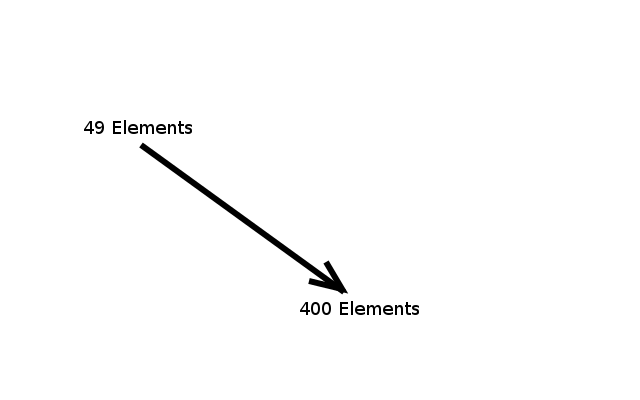
\includegraphics[scale=0.35]{arrow}};  
       \node (fig1) at (0,0)
      {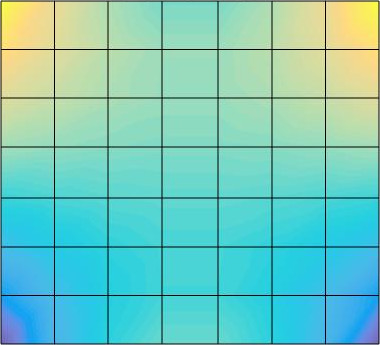
\includegraphics[scale=0.3]{uy_7^2}};
      \node (fig2) at (10,-10)
    {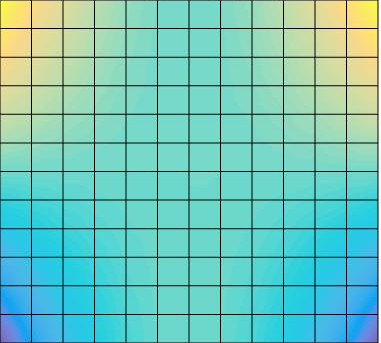
\includegraphics[scale=0.3]{uy_12^2}};
       \node (fig2) at (20,-20)
       {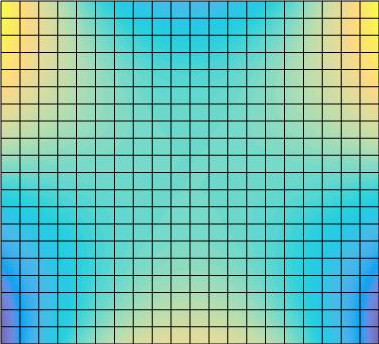
\includegraphics[scale=0.3]{uy_20^2}};  
    \end{tikzpicture}
\end{subfigure}
\begin{subfigure}{.5\textwidth}
        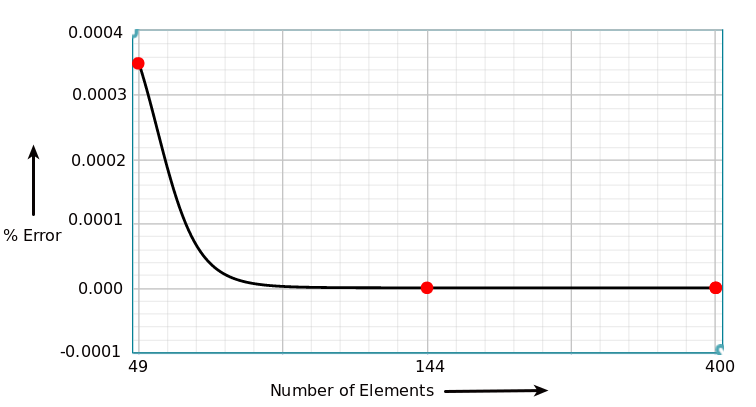
\includegraphics[scale=.28]{w}
    \end{subfigure}
\end{figure}
 \vspace{-1cm}\begin{figure}
   \centering 
  \caption{\scriptsize Errors obtained on node 30 after mesh refinements }
  \vspace{-.2cm}
 \scalebox{.8}{\begin{tabular}{|c|c|c|}
        \hline
       Number of Elements & \% Error in displacement $u_x$& \% Error in displacement $u_y$\\
        \hline
       $7\times 7$ & $0.00034894013$ & $0.00034894013$ \\
        \hline
         $12\times 12$ & $1.764697\times 10^{-7}$ & $1.764697\times 10^{-7}$ \\
        \hline
        $20\times 20$ & $1.265804\times 10^{-8}$ & $1.265804\times 10^{-8}$ \\
        \hline
    \end{tabular}}
\end{figure}
\end{frame}

%%%%%%%%%%%%%%%%%%%%%%%%%%%%%%%%%%%%%%%%%%%%%%%%%%%%%%%%%%%%%%%%%%%%%%% 
\begin{frame}[t,fragile]{Plate with edge crack}
    \vspace{-20pt} 
\begin{figure}
    \begin{subfigure}{.2\textwidth}
         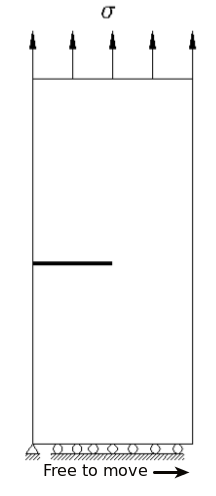
\includegraphics[scale=.20]{3.png}
         \caption{\scriptsize Edge crack}
    \end{subfigure}
    \hspace{15pt}
    \begin{subfigure}{.2\textwidth}
    \vspace{15pt}
              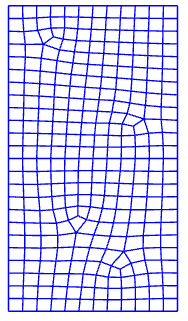
\includegraphics[scale=.22]{untitled1.png}
            \caption{\scriptsize Mesh configuration}
    \end{subfigure}
    \begin{subfigure}{.5\textwidth}
    \vspace{10pt}
         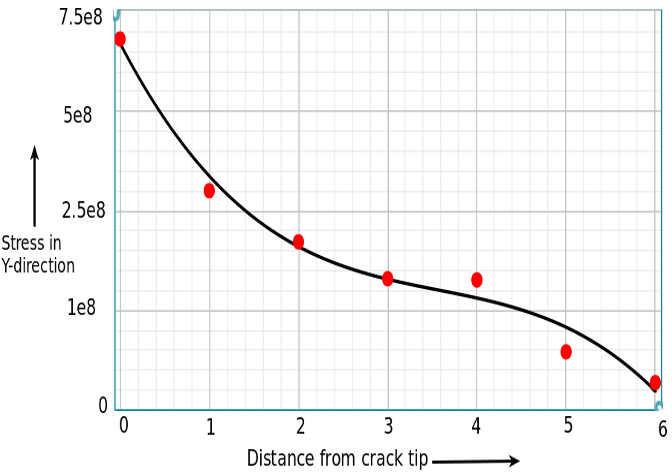
\includegraphics[scale=.25]{z}
        \vspace{-5pt}
         \caption{\scriptsize $\sigma_y$ ahead of the crack tip}
    \end{subfigure}
\end{figure}
    \vspace{-10pt}
\begin{itemize}
        \scriptsize
     \item An edge crack problem is solved applying stress $\sigma_y=100$ Mpa and taking E=200 Gpa and $\nu$=0.3.
     \item Stress intensity factor is calculated using the crack closure integral technique. 
     \item Same problem is solved in X-FEM program developed by Parnaik and compared by our solution 
\end{itemize}
\tiny
   \hspace{15pt}
    \textbf{source}:  Koustubh Parnaik. (2013). Implementation of Extended Finite Element Method (X-FEM) for static\\
   \hspace{15pt}fracture problems.
\emph{Department of Mechanical Engineering, IIT Bombay}.

\end{frame}
%%%%%%%%%%%%%%%%%%%%%%%%%%%%%%%%%%%%%%%%%%%%%%%%%%%%%%%%%%%%%%%5
\begin{frame}[t,fragile]{Comparison of FEM and X-FEM methods}
    \vspace{-.9cm}
    \hspace{15pt}
        \begin{figure}[H]
  \begin{subfigure}{0.45\textwidth}
    \centering
       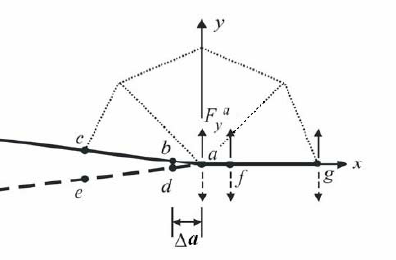
\includegraphics[scale=.2]{crackclosure.png}
    \caption{\tiny Crack closure technique}
\end{subfigure}
        \hspace{15pt}
      \begin{subfigure}{0.45\textwidth}
    \centering
        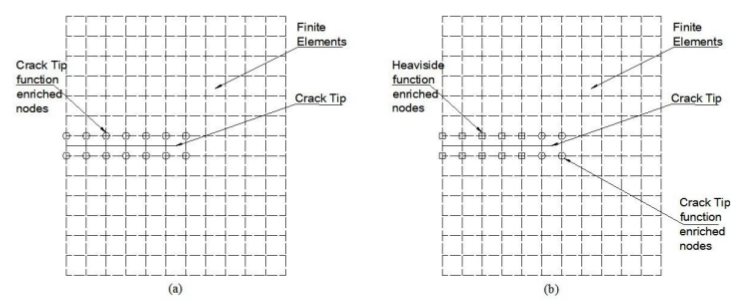
\includegraphics[scale=.15]{k.png}
    \caption{\tiny X-FEM enrichment of nodes}
\end{subfigure}
\end{figure}
\vspace{-12pt}
    \tiny    
$$
        \text{Crack closure integral:}\ \ \ \ \ \ \ G_I=\frac{W}{B\Delta a}=\frac{F_{y}^au_{y}^b}{2B \Delta a}\ \ \ \
    Thus, \ \ \ \
    K_I=\sqrt{\frac{G_I}{E}}=5.24586910\times 10^9\ \ Pa\sqrt{m}$$ $$ 
       \text{Analytical:}\ \ \ \ \ \ \ K_I=C*\sigma\sqrt{\pi a}=4.726065 \times 10^9\ \ Pa\sqrt{m}
    $$
\vspace{-10pt}
\bgroup 
\def\arraystretch{2}   
\begin{table}[H]
    \centering
    \begin{tabular}{|C{3cm}|C{6cm}|}
\hline 
Method used& $\% \ Error= \{K_{theoretical}-K_{numerical}/K_{theoretical}\}\times 100$\\
\hline
 Finite Element Method & 11.1\%\\
\hline
 Extended Finite Element Method& 4\%\\
\hline
\end{tabular}
\label{table1}
\end{table}
\egroup
\tiny
    \vspace{-.1cm}
   \hspace{15pt}
     \textbf{source}:Kumar, P., \& Prashant, K. (2009). Elements of fracture mechanics. Tata McGraw-Hill Education.
      
\end{frame} 
%%%%%%%%%%%%%%%%%%%%%%%%%%%%%%%%%%%%%%%%%%%%%%%%%%%%%%%%%%%%%%%
\begin{frame}[t,fragile]{Conclusions and Future Work}
    \vspace{-.2cm}
\begin{itemize}
             \item Conclusions:
\begin{itemize}
             \item Finite Element Formulation of semi-coupled thermoelasticity is performed. 
         \item MATLAB program is developed based on the semi-coupled formulation.
         \item Patch tests were performed to validate the FEM program.
         \item Results of FEM and X-FEM programs were compared and it is shown that solution improves when X-FEM is used. 
   \end{itemize} 
         \item Future work:
\begin{itemize}
  \item Finite Element Formulation of Fully-coupled problems 
           \item Application of the Extended Finite Element enrichments to both displacement and temperature fields  
             \item Utilization of the X-FEM program in other fields which is governed by the Laplace's equation.
    \end{itemize}
   \end{itemize} 
\end{frame}
%%%%%%%%%%%%%%%%%%%%%%%%%%%%%%%%%%%%%%%%%%%%%%%%%%%%%%%%%%%%%%%%%
\begin{frame}
    \centering
    \textbf{\huge{Thank You!}}
\end{frame}
\end{document}
